\section{Indução eletromagnética}

\frame{
	\frametitle{Indução eletromagnética}
	\begin{block}{Introdução}
		Em 1820, Hans Christian Oersted descobriu que a passagem de uma corrente elétrica em um condutor mudava a direção da agulha de uma bússola. Ou seja, ele descobriu o \textbf{eletromagnetismo}.
		\begin{itemize}
			\item A partir daí, muitos cientistas começaram a investigar mais profundamente a conexão entre os fenômenos elétricos e magnéticos. Eles buscavam, principalmente, descobrir se o efeito contrário era possível, isto é, se \textbf{os efeitos magnéticos poderiam gerar uma corrente elétrica}.
		\end{itemize}
	\end{block}
}

\frame{
	\frametitle{Indução eletromagnética}
	\begin{block}{Descoberta}
		Assim, em 1831, \textbf{Michael Faraday} com base em resultados experimentais, descobriu o fenômeno da \textbf{indução eletromagnética}.
		\begin{itemize}
			\item A \textbf{Lei de Faraday} e a \textbf{Lei de Lenz} são duas leis fundamentais do eletromagnetismo e determinam a \textbf{indução eletromagnética}.
		\end{itemize}
	\end{block}
}

\frame{
	\frametitle{Indução eletromagnética}
	\begin{block}{Definição}
		Indução eletromagnética é o fenômeno relacionado ao \textbf{aparecimento de uma corrente elétrica} em um condutor imerso em um campo magnético, \textbf{quando ocorre variação do fluxo} que o atravessa.
	\end{block}
}

\frame{
	\frametitle{Indução eletromagnética}
	\begin{block}{Definição}
		Podemos dizer que com uma simples movimentação de um ímã próximo a uma espira é possível produzir corrente elétrica. A produção de corrente elétrica por campos magnéticos recebeu o nome de \textbf{indução eletromagnética} e a corrente gerada por meio desse processo é chamada de \textbf{corrente induzida}.
	\end{block}

	\centering
	\setmyunit{1.5cm}
	\begin{tikzpicture}[scale=0.5]
			\draw (-4,-3) rectangle (4,3); %CLP
		\draw (-4,0) -- (-2.5,0); %Div in out
		\draw (-2.5,-3) -- (-2.5,3); %Div cartoes
		\draw (-1.5,-2.5) rectangle (0,2.5); %Mem dados
		\draw (0.5,-2.5) rectangle (3.5,-1); %Mem prog
		\draw (1,0) rectangle (3,2); %CPU
		\draw (-4,-5) rectangle (4,-3); %Alimentacao
		\draw (-2.5,4) rectangle (4,6); %Term de prog
		
		\draw (1,2.6) node {CLP};
		
		\draw (-3.25,1.5) node[text width=1.5cm,align=center,rotate=90] {\small Cartões de input};
		
		\draw (-3.25,-1.5) node[text width=1.5cm,align=center,rotate=90] {\small Cartões de output};
		
		\node at (2,1) {\small CPU};
		
		\node[rotate=90,text width=1.5cm,align=center] at (-0.75,0) {\small Memória de dados};
		
		\node[text width=2cm,align=center] at (2,-1.75) {\footnotesize Memória de programa};
		
		\node at (-6,0) {Campo};
		
		\node at (0,-4) {Alimentação};
		
		\node[text width=3cm,align=center] at (0.75,5) {Terminal de programação};
		
		\draw[-Latex] (-8,1.5) -- node[above] {Entradas} +(4,0);
		\draw[Latex-] (-8,-1.5) -- node[below] {Saídas} +(4,0);
		\draw[-Latex] (-2.5,1.5) -- +(1,0);
		\draw[Latex-] (-2.5,-1.5) -- +(1,0);
		\draw[-Latex] (0,1.5) -- +(1,0);
		\draw[Latex-] (0,0.5) -- +(1,0);
		\draw[Latex-] (2,0) -- +(0,-1);
		
		\draw[-Latex] (-1.5,4) -- +(0,-1);
		\draw[Latex-] (3,4) -- +(0,-1);
	\end{tikzpicture}
%	\centerline{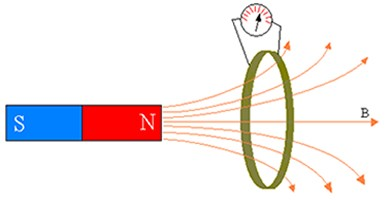
\includegraphics[width=0.6\linewidth]{Figuras/Ch10/fig1.jpg}}
}

\frame{
	\frametitle{Fluxo magnético}
	\begin{block}{Introdução}
		Para que se entenda o que é, e como se origina a indução eletromagnética é necessário que definamos uma grandeza física chamada \textbf{fluxo magnético}. Esta grandeza é vetorial é simbolizada por $\vec{\Phi}$.
	\end{block}
}

\frame{
	\frametitle{Fluxo magnético}
	\begin{block}{Definição}
		Podemos escrever o fluxo magnético como o produto do vetor indução magnética (campo magnético) $\vec{B}$ pela área da superfície $A$ e pelo cosseno do ângulo $\theta$, formado entre e uma linha perpendicular à superfície, chamada reta normal.
		$$\boxed{\vec{\Phi} = B \cdot A \cdot \cos \theta}$$
		\begin{itemize}
			\item A unidade adotada para se medir o fluxo de indução magnética pelo SI é o \textbf{Weber} (Wb), em homenagem ao físico alemão Wilhelm Webber, e caracteriza Tesla por metro quadrado (T/m$^2$).
		\end{itemize}
	\end{block}
}

\frame{
	\frametitle{Fluxo magnético}
	\begin{block}{Definição}
		\begin{itemize}
			\item É possível também se associar o fluxo de indução magnética à \textbf{quantidade de linhas de indução que atravessam a superfície}.
		\end{itemize}
	\end{block}
%	\vspace{0.5cm}

	\centering
	
	\setmyunit{1cm}
	\begin{tikzpicture}
	\foreach \x in {-1.5,-1,...,1.5}
	\draw[blue] (0,\x) -- +(2,0);
	
	\draw (5.5,0) node[blue] {$ \vec{B} $};
	
	\filldraw[fill=black!40!white,draw=black,rotate=-30] (2,1) circle (1.5 and 0.5);
	
	\foreach \x in {-1.5,-1,1,1.5}
	\draw[-Latex,blue] (2,\x) -- +(3,0);
	
	\draw[-Latex,blue] (1.5,0.5) -- (5,0.5);
	\draw[-Latex,blue,name path=midb] (2.2,0) -- (5,0);
	\draw[-Latex,blue] (2.8,-0.5) -- (5,-0.5);
	
	\draw[rotate=-30] (2,1) rectangle +(0.1,0.1) node[pos=.5] {$ \cdot $};
	\draw[-Latex,rotate=-30,name path=nar] (2,1) -- node[above,rotate=60] {Reta normal} +(0,2) node[name=B,coordinate] {};
	
	\coordinate (A) at (5,0);
	\draw[name intersections={of=nar and midb, by=x}] (x) node[coordinate,name=O] {};
	
	\pic[draw,red, angle radius=8pt,angle eccentricity=1,"$ \theta $" {xshift=3pt,yshift=3pt}] {angle=A--O--B};
	\end{tikzpicture}
%	\centerline{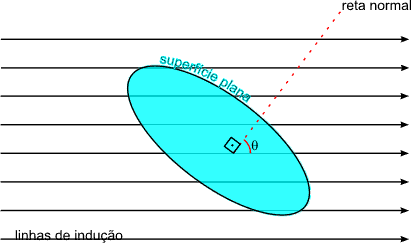
\includegraphics[width=0.6\linewidth]{Figuras/Ch10/fig2.png}}
}

\frame{
	\frametitle{Fluxo magnético}
	\begin{block}{Caso especial $\#01$}
		\begin{itemize}
			\item Se a reta normal à superfície for \textbf{perpendicular ao vetor indução magnética}, nenhuma linha de indução o atravessará, portanto o \textbf{fluxo será nulo}. Isto pode ser comprovado pela equação do fluxo magnético já que $\cos\ang{90} = 0$
		\end{itemize}
	\end{block}
%	\vspace{0.5cm}
	\centering
	
	\setmyunit{1cm}
	\begin{tikzpicture}
	\foreach \x in {-1.5,-1,...,1.5}
	\draw[blue] (0,\x) -- +(2,0);
	
	\draw (5.5,0) node[blue] {$ \vec{B} $};
	
	\filldraw[fill=black!40!white,draw=black] (2,0) circle (1.5 and 0.5);
	
	\foreach \x in {-1.5,-1,...,1.5}
	\draw[-Latex,blue] (2,\x) -- +(3,0);
	
	\draw[red] (2.1,0) rectangle +(0.1,0.1) node[pos=.5] {$ \cdot $};
	\draw (2,0) rectangle +(0.1,0.1) node[pos=.5] {$ \cdot $};
	\draw[-Latex] (2,0) -- node[above,rotate=90] {Reta normal} +(0,2);
	\end{tikzpicture}
	
%	\centerline{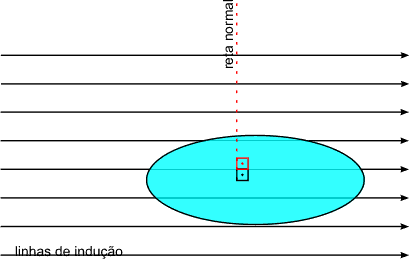
\includegraphics[width=0.6\linewidth]{Figuras/Ch10/fig3.png}}
}

\frame{
	\frametitle{Fluxo magnético}
	\begin{block}{Caso especial $\#02$}
		\begin{itemize}
			\item Se a reta normal à superfície for \textbf{paralela ao vetor indução magnética}, o número máximo de linhas de indução o atravessará, portanto o \textbf{fluxo será máximo}. Isto pode ser comprovado pela equação do fluxo magnético já que $\cos\ang{0} = 1$
		\end{itemize}
	\end{block}
%	\vspace{0.5cm}

	\bigskip
	\centering
	
	\setmyunit{1cm}
	\begin{tikzpicture}
		\foreach \x in {-1.5,-1,...,1.5}
			\draw[,blue] (0,\x) -- +(1,0);
		
		\draw (4.5,0) node[blue] {$ \vec{B} $};
		
		\filldraw[fill=black!40!white,draw=black] (1,0) circle (0.5 and 1.5);
		
		\foreach \x in {-1.5,-1,...,1.5}
			\draw[-Latex,blue] (1,\x) -- +(3,0);
		
		\draw (1,0) rectangle +(0.1,-0.1) node[pos=.5] {$ \cdot $};
		\draw[-Latex] (1,0) -- node[above] {Reta normal} +(2,0);
	\end{tikzpicture}
	
%	

\tikzset{every picture/.style={line width=0.75pt}} %set default line width to 0.75pt        

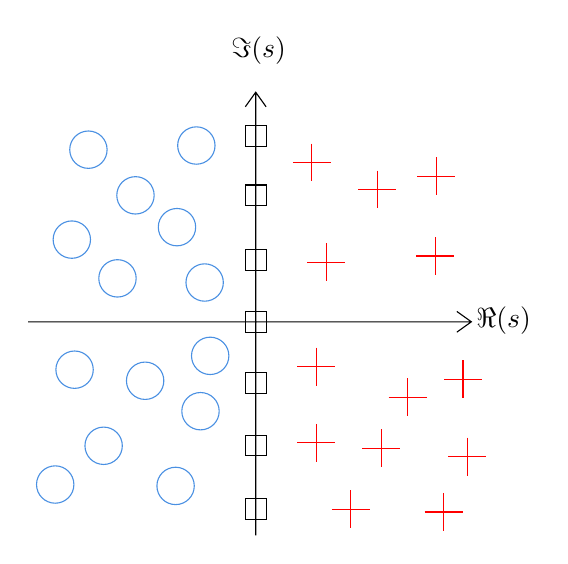
\begin{tikzpicture}[x=0.75pt,y=0.75pt,yscale=-1,xscale=1]
%uncomment if require: \path (0,300); %set diagram left start at 0, and has height of 300

%Shape: Axis 2D [id:dp27678030181731494] 
\draw  (40,160.6) -- (253.5,160.6)(149.6,50) -- (149.6,263.5) (246.5,155.6) -- (253.5,160.6) -- (246.5,165.6) (144.6,57) -- (149.6,50) -- (154.6,57)  ;
%Shape: Square [id:dp29640104318485094] 
\draw   (144.6,155.6) -- (154.6,155.6) -- (154.6,165.6) -- (144.6,165.6) -- cycle ;
%Shape: Square [id:dp5015049228757054] 
\draw   (144.6,125.7) -- (154.6,125.7) -- (154.6,135.7) -- (144.6,135.7) -- cycle ;
%Shape: Square [id:dp5724308304859749] 
\draw   (144.6,94.7) -- (154.6,94.7) -- (154.6,104.7) -- (144.6,104.7) -- cycle ;
%Shape: Square [id:dp8722658997981245] 
\draw   (144.6,66.2) -- (154.6,66.2) -- (154.6,76.2) -- (144.6,76.2) -- cycle ;
%Shape: Square [id:dp035501458242915174] 
\draw   (144.6,185.2) -- (154.6,185.2) -- (154.6,195.2) -- (144.6,195.2) -- cycle ;
%Shape: Square [id:dp23226558696093957] 
\draw   (144.6,215.2) -- (154.6,215.2) -- (154.6,225.2) -- (144.6,225.2) -- cycle ;
%Shape: Square [id:dp09667812864869552] 
\draw   (144.6,245.7) -- (154.6,245.7) -- (154.6,255.7) -- (144.6,255.7) -- cycle ;
\draw  [color={rgb, 255:red, 255; green, 0; blue, 0 }  ,draw opacity=1 ] (167.5,83.88) -- (185.75,83.88)(176.63,74.75) -- (176.63,93) ;
\draw  [color={rgb, 255:red, 255; green, 0; blue, 0 }  ,draw opacity=1 ] (199,96.88) -- (217.25,96.88)(208.13,87.75) -- (208.13,106) ;
\draw  [color={rgb, 255:red, 255; green, 0; blue, 0 }  ,draw opacity=1 ] (174.5,131.88) -- (192.75,131.88)(183.63,122.75) -- (183.63,141) ;
\draw  [color={rgb, 255:red, 255; green, 0; blue, 0 }  ,draw opacity=1 ] (227,128.88) -- (245.25,128.88)(236.13,119.75) -- (236.13,138) ;
\draw  [color={rgb, 255:red, 255; green, 0; blue, 0 }  ,draw opacity=1 ] (227.5,90.38) -- (245.75,90.38)(236.63,81.25) -- (236.63,99.5) ;
\draw  [color={rgb, 255:red, 255; green, 0; blue, 0 }  ,draw opacity=1 ] (169.67,182.21) -- (187.92,182.21)(178.79,173.08) -- (178.79,191.33) ;
\draw  [color={rgb, 255:red, 255; green, 0; blue, 0 }  ,draw opacity=1 ] (186.33,250.88) -- (204.58,250.88)(195.46,241.75) -- (195.46,260) ;
\draw  [color={rgb, 255:red, 255; green, 0; blue, 0 }  ,draw opacity=1 ] (231,252.21) -- (249.25,252.21)(240.13,243.08) -- (240.13,261.33) ;
\draw  [color={rgb, 255:red, 255; green, 0; blue, 0 }  ,draw opacity=1 ] (169.67,218.88) -- (187.92,218.88)(178.79,209.75) -- (178.79,228) ;
\draw  [color={rgb, 255:red, 255; green, 0; blue, 0 }  ,draw opacity=1 ] (242.33,225.54) -- (260.58,225.54)(251.46,216.42) -- (251.46,234.67) ;
\draw  [color={rgb, 255:red, 255; green, 0; blue, 0 }  ,draw opacity=1 ] (213.67,196.88) -- (231.92,196.88)(222.79,187.75) -- (222.79,206) ;
\draw  [color={rgb, 255:red, 255; green, 0; blue, 0 }  ,draw opacity=1 ] (240.33,188.21) -- (258.58,188.21)(249.46,179.08) -- (249.46,197.33) ;
\draw  [color={rgb, 255:red, 255; green, 0; blue, 0 }  ,draw opacity=1 ] (201,221.54) -- (219.25,221.54)(210.13,212.42) -- (210.13,230.67) ;
%Shape: Circle [id:dp01739200493370019] 
\draw  [color={rgb, 255:red, 74; green, 144; blue, 226 }  ,draw opacity=1 ] (60,77.67) .. controls (60,72.7) and (64.03,68.67) .. (69,68.67) .. controls (73.97,68.67) and (78,72.7) .. (78,77.67) .. controls (78,82.64) and (73.97,86.67) .. (69,86.67) .. controls (64.03,86.67) and (60,82.64) .. (60,77.67) -- cycle ;
%Shape: Circle [id:dp857755141402053] 
\draw  [color={rgb, 255:red, 74; green, 144; blue, 226 }  ,draw opacity=1 ] (82.67,99.67) .. controls (82.67,94.7) and (86.7,90.67) .. (91.67,90.67) .. controls (96.64,90.67) and (100.67,94.7) .. (100.67,99.67) .. controls (100.67,104.64) and (96.64,108.67) .. (91.67,108.67) .. controls (86.7,108.67) and (82.67,104.64) .. (82.67,99.67) -- cycle ;
%Shape: Circle [id:dp9246833060771249] 
\draw  [color={rgb, 255:red, 74; green, 144; blue, 226 }  ,draw opacity=1 ] (44,239) .. controls (44,234.03) and (48.03,230) .. (53,230) .. controls (57.97,230) and (62,234.03) .. (62,239) .. controls (62,243.97) and (57.97,248) .. (53,248) .. controls (48.03,248) and (44,243.97) .. (44,239) -- cycle ;
%Shape: Circle [id:dp8304441936419562] 
\draw  [color={rgb, 255:red, 74; green, 144; blue, 226 }  ,draw opacity=1 ] (118.67,177) .. controls (118.67,172.03) and (122.7,168) .. (127.67,168) .. controls (132.64,168) and (136.67,172.03) .. (136.67,177) .. controls (136.67,181.97) and (132.64,186) .. (127.67,186) .. controls (122.7,186) and (118.67,181.97) .. (118.67,177) -- cycle ;
%Shape: Circle [id:dp5059258663614863] 
\draw  [color={rgb, 255:red, 74; green, 144; blue, 226 }  ,draw opacity=1 ] (102.67,115) .. controls (102.67,110.03) and (106.7,106) .. (111.67,106) .. controls (116.64,106) and (120.67,110.03) .. (120.67,115) .. controls (120.67,119.97) and (116.64,124) .. (111.67,124) .. controls (106.7,124) and (102.67,119.97) .. (102.67,115) -- cycle ;
%Shape: Circle [id:dp21245040687156935] 
\draw  [color={rgb, 255:red, 74; green, 144; blue, 226 }  ,draw opacity=1 ] (52,121) .. controls (52,116.03) and (56.03,112) .. (61,112) .. controls (65.97,112) and (70,116.03) .. (70,121) .. controls (70,125.97) and (65.97,130) .. (61,130) .. controls (56.03,130) and (52,125.97) .. (52,121) -- cycle ;
%Shape: Circle [id:dp17429736806925722] 
\draw  [color={rgb, 255:red, 74; green, 144; blue, 226 }  ,draw opacity=1 ] (116,141.67) .. controls (116,136.7) and (120.03,132.67) .. (125,132.67) .. controls (129.97,132.67) and (134,136.7) .. (134,141.67) .. controls (134,146.64) and (129.97,150.67) .. (125,150.67) .. controls (120.03,150.67) and (116,146.64) .. (116,141.67) -- cycle ;
%Shape: Circle [id:dp33160849295458217] 
\draw  [color={rgb, 255:red, 74; green, 144; blue, 226 }  ,draw opacity=1 ] (74,139.67) .. controls (74,134.7) and (78.03,130.67) .. (83,130.67) .. controls (87.97,130.67) and (92,134.7) .. (92,139.67) .. controls (92,144.64) and (87.97,148.67) .. (83,148.67) .. controls (78.03,148.67) and (74,144.64) .. (74,139.67) -- cycle ;
%Shape: Circle [id:dp32709834546378724] 
\draw  [color={rgb, 255:red, 74; green, 144; blue, 226 }  ,draw opacity=1 ] (87.33,189) .. controls (87.33,184.03) and (91.36,180) .. (96.33,180) .. controls (101.3,180) and (105.33,184.03) .. (105.33,189) .. controls (105.33,193.97) and (101.3,198) .. (96.33,198) .. controls (91.36,198) and (87.33,193.97) .. (87.33,189) -- cycle ;
%Shape: Circle [id:dp8791724327388495] 
\draw  [color={rgb, 255:red, 74; green, 144; blue, 226 }  ,draw opacity=1 ] (53.33,183.67) .. controls (53.33,178.7) and (57.36,174.67) .. (62.33,174.67) .. controls (67.3,174.67) and (71.33,178.7) .. (71.33,183.67) .. controls (71.33,188.64) and (67.3,192.67) .. (62.33,192.67) .. controls (57.36,192.67) and (53.33,188.64) .. (53.33,183.67) -- cycle ;
%Shape: Circle [id:dp4794866171308949] 
\draw  [color={rgb, 255:red, 74; green, 144; blue, 226 }  ,draw opacity=1 ] (114,203.67) .. controls (114,198.7) and (118.03,194.67) .. (123,194.67) .. controls (127.97,194.67) and (132,198.7) .. (132,203.67) .. controls (132,208.64) and (127.97,212.67) .. (123,212.67) .. controls (118.03,212.67) and (114,208.64) .. (114,203.67) -- cycle ;
%Shape: Circle [id:dp5349657045143856] 
\draw  [color={rgb, 255:red, 74; green, 144; blue, 226 }  ,draw opacity=1 ] (67.33,220.33) .. controls (67.33,215.36) and (71.36,211.33) .. (76.33,211.33) .. controls (81.3,211.33) and (85.33,215.36) .. (85.33,220.33) .. controls (85.33,225.3) and (81.3,229.33) .. (76.33,229.33) .. controls (71.36,229.33) and (67.33,225.3) .. (67.33,220.33) -- cycle ;
%Shape: Circle [id:dp714149478603834] 
\draw  [color={rgb, 255:red, 74; green, 144; blue, 226 }  ,draw opacity=1 ] (102,239.67) .. controls (102,234.7) and (106.03,230.67) .. (111,230.67) .. controls (115.97,230.67) and (120,234.7) .. (120,239.67) .. controls (120,244.64) and (115.97,248.67) .. (111,248.67) .. controls (106.03,248.67) and (102,244.64) .. (102,239.67) -- cycle ;
%Shape: Circle [id:dp476022910470574] 
\draw  [color={rgb, 255:red, 74; green, 144; blue, 226 }  ,draw opacity=1 ] (112,75.67) .. controls (112,70.7) and (116.03,66.67) .. (121,66.67) .. controls (125.97,66.67) and (130,70.7) .. (130,75.67) .. controls (130,80.64) and (125.97,84.67) .. (121,84.67) .. controls (116.03,84.67) and (112,80.64) .. (112,75.67) -- cycle ;

% Text Node
\draw (151,30) node   {$\Im(s)$};
% Text Node
\draw (269,160) node   {$\Re(s)$};


\end{tikzpicture}
%	\centerline{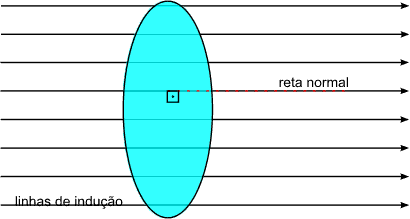
\includegraphics[width=0.6\linewidth]{Figuras/Ch10/fig4.png}}
}

\frame{
	\frametitle{Lei de Faraday}
	\begin{block}{Introdução}
		Quando o fluxo magnético através da superfície de uma espira varia, surge na espira uma corrente elétrica induzida. Havendo corrente elétrica induzida no circuito, concluímos que deve haver uma \textbf{força eletromotriz induzida} que a originou.
		\begin{itemize}
			\item Experimentalmente, Faraday observou que, quanto mais rápida é a variação do fluxo magnético $\vec{\Phi}$, maior é a força eletromotriz induzida. Estabeleceu, então, que a \textbf{força eletromotriz induzida} ($\varepsilon$) \textbf{é proporcional à rapidez com que o fluxo magnético varia}. \\
		\end{itemize}
		$$\boxed{\vec{\varepsilon} = \dfrac{\Delta \vec{\Phi}}{\Delta t}}$$
	\end{block}
}

\frame{
	\frametitle{Lei de Faraday - Exemplo \#01}
	\begin{block}{}
		Uma espira plana de área $A = \SI{3.0e-3}{\meter\squared}$ está colocada paralelamente às linhas de indução de um campo magnético uniforme de intensidade $|\vec{B}| = \SI{8.0e-2}{\tesla}$. Gira-se a espira e, após um intervalo de tempo $\Delta t = \SI{0.40}{\second}$, a espira fica perpendicular às linhas de indução. Determine, nesse intervalo de tempo, o valor absoluto da fem.
	\end{block}
}

\frame{
	\frametitle{Lei de Faraday - Exemplo \#01}
	\begin{block}{Resolução}
		\begin{itemize}
			\item Para o instante $t = \SI{0}{\second}$: \\
			      \vspace{0.2cm}
			      $\vec{\Phi} = B \cdot A \cdot \cos \theta = B \cdot A \cdot \cos \ang{90} = \SI{0}{\weber}$
			\item Para o instante $t = \SI{0.4}{\second}$: \\
			      \vspace{0.2cm}
			      $\vec{\Phi} = B \cdot A \cdot \cos \theta = \num{8.0e-2} \cdot \num{3.0e-3} \cdot \cos\ang{0} = \SI{2.4e-4}{\weber}$
		\end{itemize}
		\vspace{0.4cm}
		Deste modo, $\vec{\varepsilon} = \dfrac{\Delta \vec{\Phi}}{\Delta t} = \dfrac{\num{2.4e-4} - 0}{\num{0.4} - 0} = \SI{6e-4}{\volt}$
	\end{block}
}

\frame{
	\frametitle{Lei de Lenz}
	\begin{block}{Introdução}
		Apesar de identificar que a corrente induzida variava de sentido, \textbf{Faraday não conseguiu determinar como ocorria essa variação}.
		\begin{itemize}
			\item Então em 1834, o físico russo Heinrich Lenz, propôs uma regra para a \textbf{definição do sentido da corrente induzida}.
		\end{itemize}
	\end{block}
}

\frame{
	\frametitle{Lei de Lenz}
	\begin{block}{A Lei}
		\textbf{``O sentido da corrente elétrica induzida é tal que seus efeitos (campo magnético produzido) se opõem à causa que lhe deu origem (variação do fluxo magnético que a produziu).''}
		\begin{itemize}
			\item Essa lei é representada na fórmula da força eletromotriz induzida através do \textbf{sinal de menos}.
			      $$\boxed{\vec{\varepsilon} = -\dfrac{\Delta \vec{\Phi}}{\Delta t}}$$
			\item Isso significa que \textbf{qualquer campo magnético produzido por uma corrente induzida será na direção oposta à variação do campo original}. Este resultado é frequentemente chamado de \textbf{Lei de Faraday-Lenz}.
		\end{itemize}
	\end{block}
}

\frame{
	\frametitle{Lei de Lenz}
	\begin{block}{A Lei}
		Em outras palavras: se o fluxo aumentou, a corrente vai querer que o fluxo diminua; se o fluxo diminuiu, a corrente vai querer que o fluxo aumente.
	\end{block}
	\centerline{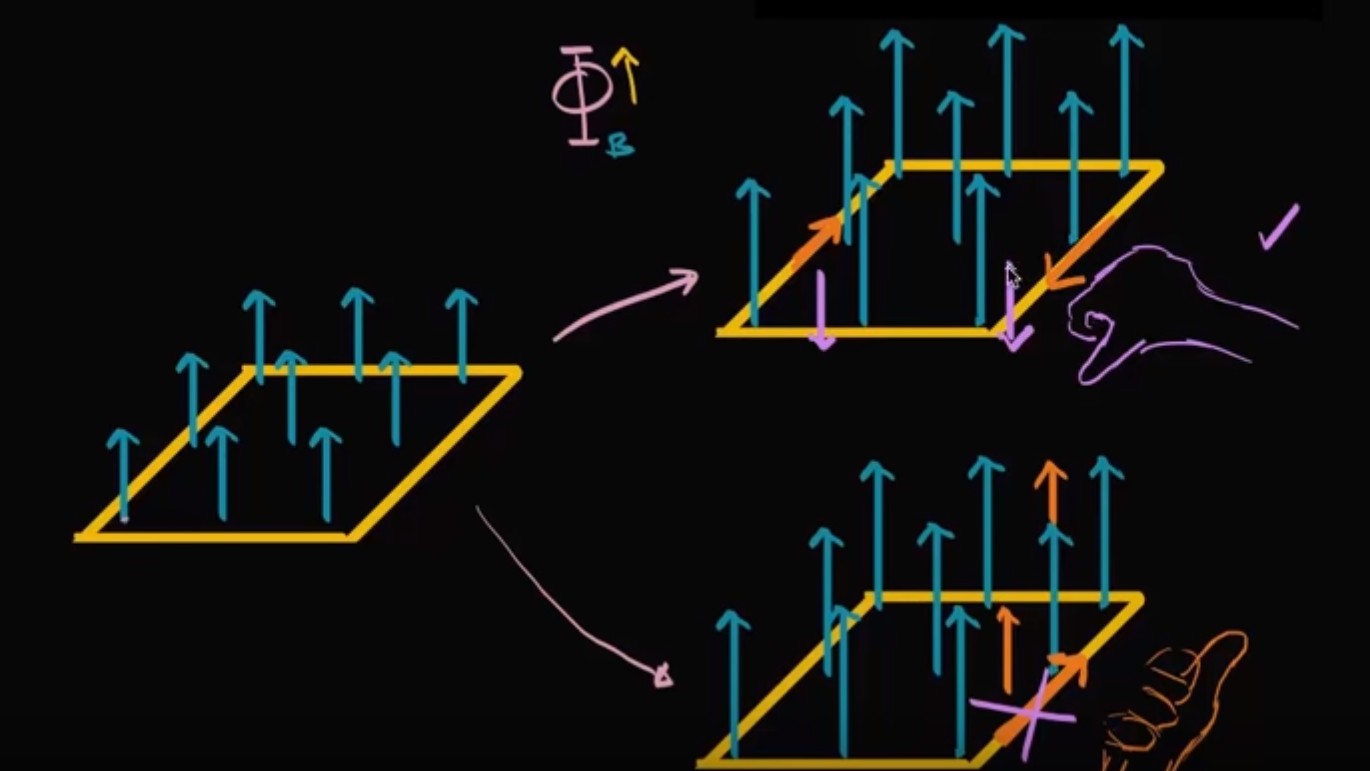
\includegraphics[width=0.8\linewidth]{Figuras/Ch10/fig5.PNG}}
}

\frame{
	\frametitle{Lei de Lenz}
	\begin{block}{A Lei}
		Com essa afirmação pode-se concluir que quando um ímã é aproximado de uma espira, por exemplo, ele será repelido; e quando se afastar ele será atraído.
	\end{block}
	\centerline{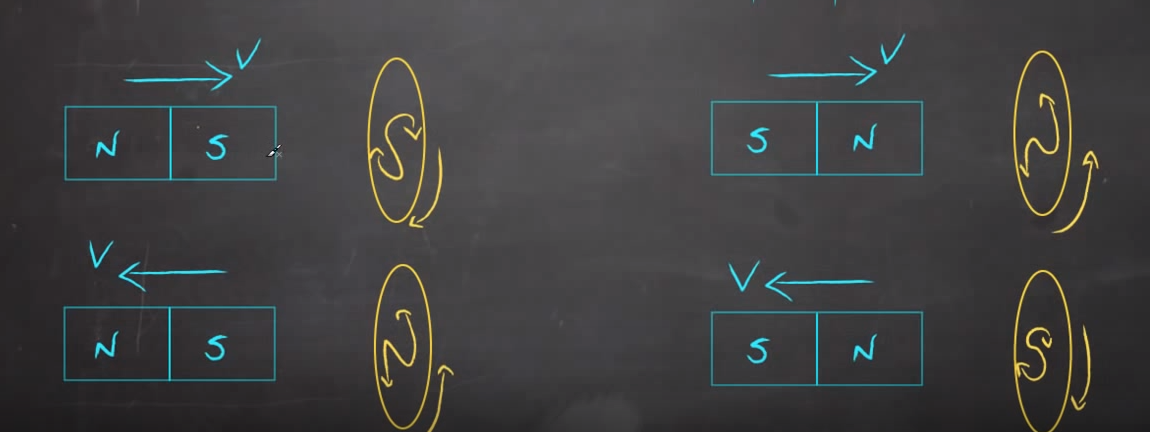
\includegraphics[width=1\linewidth]{Figuras/Ch11/lenz.PNG}}
}

\frame{
	\frametitle{Transformadores}
	\begin{block}{Introdução}
		A energia elétrica após ser produzida nas usinas é transportada para os centros consumidores através de sistemas de transmissão. Contudo, antes de ser transportada para grandes distâncias, os dispositivos, chamados de \textbf{transformadores}, \textbf{elevam a tensão} para reduzir as perdas de energia. Quando essa energia chega até o seu destino final, \textbf{novamente ocorrerá a mudança no valor da tensão}.
		\begin{itemize}
			\item Assim, um \textbf{transformador é um dispositivo que serve para modificar uma tensão alternada, ou seja, aumenta ou diminui o seu valor de acordo com a necessidade}.
		\end{itemize}
	\end{block}
}

\frame{
	\frametitle{Transformadores}
	\begin{block}{Princípio de funcionamento}
		Um transformador é constituído por um núcleo de material ferromagnético no qual são enroladas \textbf{duas bobinas independentes}.
		\begin{itemize}
			\item A bobina conectada a fonte é chamada de \textbf{primário}, pois recebe a tensão que será transformada.
			\item A outra é chamada de \textbf{secundário}.
			\item Como a corrente que chega no primário é alternada, origina um \textbf{fluxo magnético} também alternado no núcleo do transformador. Essa variação do fluxo, gera uma \textbf{corrente alternada induzida no secundário}.
		\end{itemize}
	\end{block}
}

\frame{
	\frametitle{Transformadores}
	\begin{block}{Princípio de funcionamento}
		O aumento ou a diminuição da tensão induzida, \textbf{depende da relação entre o número de espiras nas duas bobinas}.
		\begin{itemize}
			\item Se o número de espiras no secundário for maior que no primário o transformador irá \textbf{elevar a tensão} e sendo ao contrário, ele irá \textbf{abaixar a tensão}.
		\end{itemize}
		$$\dfrac{V_p}{V_s} = \dfrac{N_p}{N_s}$$
	\end{block}
}

\frame{
	\frametitle{Transformadores}
	\centering
	\setmyunit{1cm}
	
	\newcommand{\innercolor}{gray!70!white}
	\newcommand{\outercolor}{gray!40!white}
	\newcommand{\leftcoil}{red!75!gray}
	\pgfmathsetmacro{\coilseparation}{0.02}
	
	\pgfmathsetmacro{\halflinewidth}{0.008}
	
	
	\begin{tikzpicture}[x={(\xx*1cm,\xy*1cm)},y={(\yx*1cm,\yy*1cm)},z={(\zx*1cm,\zy*1cm)}]
	\draw[\leftcoil, thick] (-0.02,5,1.125) -- +(0,2,0) (1.02,5,3.875) -- +(0,2,0);
	
	\draw[dashed,<->] ($ (-0.02,5,1.125)+(0,2,0) $) -- ($ (1.02,5,3.875)+(0,2,0) $);
	\node[rotate=85] at ($ (-0.02,5+2,1.125)!0.5!(1.02,5+2,3.875)+(0,0.2,0) $) {$ V_p $};
	
	\draw[-latex] (-0.02,6.5,1.325) -- node[above] {$ i_p $} +(0,-1,0);
	\draw[latex-] (1.02,0.02-0.5,1.3) -- node[above] {$ i_s $} +(0,-1,0);
	
	\filldraw[fill=\innercolor]  (0,1,1) -- (1,1,1) -- (1,4,1) -- (0,4,1) -- cycle;
	\filldraw[fill=\innercolor]  (1,4,1) -- (0,4,1) -- (0,4,4) -- (1,4,4) -- cycle;
	\filldraw[fill=\innercolor]  (0,0,0) -- (1,0,0) -- (1,0,5) -- (0,0,5) -- cycle;
	\filldraw[fill=\innercolor]  (0,0,5) -- (0,5,5) -- (1,5,5) -- (1,0,5) -- cycle;
	\filldraw[fill=\outercolor,even odd rule]    (0,0,0) -- (0,5,0) -- (0,5,5) -- (0,0,5) --cycle (0,1,1) -- (0,4,1) -- (0,4,4) -- (0,1,4) --cycle ;
	
	\begin{scope}
	\clip (0,3,1) -- (0,6,1) -- (0,6,4) -- (0,3,4);
	\foreach \z in {1.125,1.375,...,3.875}
	{   \draw[\leftcoil,thick] (0,5,\z) -- (-\coilseparation,5,\z) -- (-\coilseparation,4-\coilseparation,\z) -- (1+\coilseparation,4-\coilseparation,\z) -- (1+\coilseparation,4,\z);
	}
	\end{scope}
	
	
	\foreach \z in {1.25,1.75,...,3.75}
	{   \draw[blue,thick] (0,1,\z) -- (-\coilseparation,1,\z) -- (-\coilseparation,0-\coilseparation,\z) -- (1+\coilseparation,0-\coilseparation,\z) -- (1+\coilseparation,0,\z);
	}

	\draw[blue,thick] (1+\coilseparation,0+\coilseparation,1.1) -- +(0,-2,0) (-\coilseparation,1+\coilseparation,3.85) -- +(0,-3,0);
	
	\draw[dashed,<->] (1.02,-2+0.02,1.1) -- (-0.02,0.02-2,3.85);
	\node[rotate=-70] at ($ (1.02,-2+0.02,1.1)!0.5!(-0.02,0.02-2,3.85)+(0,-0.2,0) $) {$ V_s $};
	
	\draw[decorate,decoration={brace,amplitude=10pt},xshift=-4pt,yshift=0pt] (0,5,1.25) -- +(0,0,2.75);
	\draw[decorate,decoration={brace,amplitude=10pt},xshift=-4pt,yshift=0pt] (1.2,0,3.75) -- +(0,0,-2.6);
	\node[rotate=90] at (0,5.7,2.625) {$ N_p $ espiras};
	\node[rotate=-90] at (1.2,-0.5,2.5) {$ N_s $ espiras};
	
	\draw[dashed,postaction={decorate,decoration={markings,mark=between positions 0.1 and 1 step 0.2 with \arrow{Latex}}}] (0,4.5,0.5) -- (0,0.5,0.5) -- ++(0,0,4) -- ++(0,4,0) -- cycle;
	
	\draw[] (0,2.5,4.7)% -- +(0,-0.5,1.5)
	node[rotate=-10] {Fluxo magnético ($ \phi $)};
	
	\end{tikzpicture}
	
%	\centerline{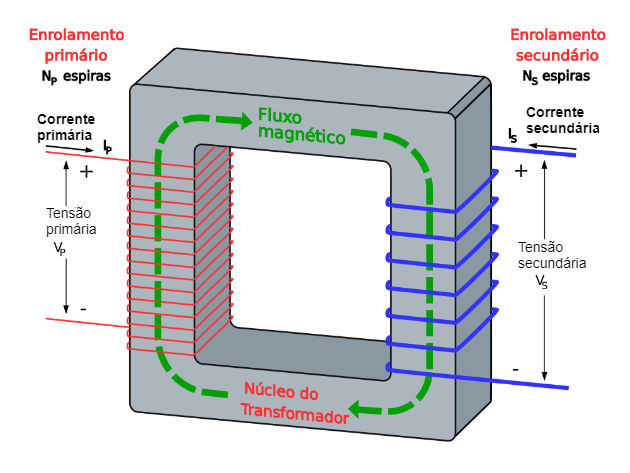
\includegraphics[width=0.9\linewidth]{Figuras/Ch10/fig6.jpg}}
}

\section*{Exercícios}
\frame{
	\frametitle{Exercícios}
	\begin{block}{}
		01. A corrente elétrica no enrolamento primário de um transformador corresponde a \SI{10}{\ampere}, enquanto no enrolamento secundário corresponde a \SI{20}{\ampere}.
		Sabendo que o enrolamento primário possui 1200 espiras, determine o número de espiras do enrolamento secundário.

		\vspace{0.5cm}

		02. Uma espira circular de raio \SI{0.2}{\meter} está sob influência de um campo magnético de módulo \SI{5}{\tesla}. Determine o fluxo magnético sobre a espira considerando que o ângulo entre o vetor campo magnético e a reta normal ao plano dessa espira seja de $\ang{60}$.
	\end{block}
}

\section*{Referências}
\frame{
	\frametitle{Referências e Exercícios Complementares}
	\begin{itemize}
		\item ALEXANDRE, Charles K.; SADIKU, Matthew N. O. Fundamentos de Circuitos Elétricos. 5. ed. Porto Alegre: AMGH, 2013.
	\end{itemize}
	%\centering{\alert{Página 36 - \textbf{1.6.1 até 1.6.5, 1.6.17 até 1.6.19}}} \\
	\centering{\alert{Lista de exercícios 10}}
}